\scanpage{13}
\deleted{\mspage{\unsure{7}}}
\mspage{12}

\deleted{
\begin{tabular}{|p{0.9\linewidth}}
\uline{Lemme} Soit $F=(X,\{A,B\})$ une ficelle, $C$ un lieu de \deleted{$\unsure{F}$ $\unsure{I}$} $F$ distinct des extrémités, \deleted{\unsure{d'}} de \deleted{ficelles} subdivision
\[
F_{A,C}=(X_{A,C},\{A,C\}),\quad F_{B,C}=(X_{\unsure{B|A},C},\{B,C\}).
\]
Soit $\unsure{B|D}$ un \deleted{partie} lieu de $F_{B,C}$, distinct des extrémités. Alors $C$ est un lieu de $F_{A,D}$, distinct des extrémités (et inverse
\end{tabular}

\figure{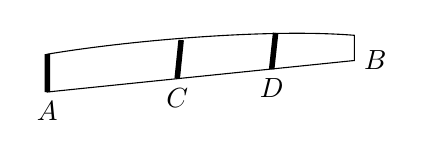
\begin{tikzpicture}[x=1cm,y=1cm]
\draw (0,0) -- (3.9,.4) -- (3.9,.72) .. controls (2.8,.81) and (1,.65) .. (0,.48) -- cycle;
\draw[line width=2pt] (0,0)--(0,.48) (1.65,.17)--(1.7,.66) (2.85,.29)--(2.9,.75);
\node[below] at (0,0){$A$}; \node[below] at (1.65,.17){$C$}; \node[below] at (2.85,.29){$D$}; \node[right] at (3.9,.4){$B$};
\end{tikzpicture}}
OPS $A,B,C,D$ réduits à des points.

\deleted{Ficelle orientée}

\diagram{\begin{tikzcd}[ampersand replacement=\&,column sep=large]
\deleted{A,C,D}\arrow[r,Rightarrow] \& {}\\
\unsure{T|I}\ D,B,C\arrow[r,Rightarrow] \& C,A,D\arrow[r,Rightarrow] \& D,B,C
\end{tikzcd}}
}

\unsure{2}) Être homéom. à $B^n$: On trouve notamment la théorie des décompositions
\figure{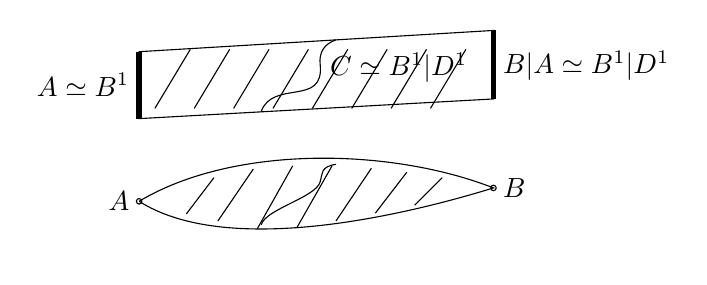
\begin{tikzpicture}[x=1cm,y=1cm]
\draw (0,0)--(4.5,.25)--(4.5,1.12)--(0,.85)--cycle;
\foreach \xa in {.2,.7,1.2,1.7,2.2,2.7,3.2,3.7}{
\draw[thin] (\xa,.13) -- (\xa+.45,.88);}
\draw[line width=2pt] (0,0)--(0,.85) (4.5,.25)--(4.5,1.12);
\draw (1.55,.09) .. controls (1.7,.5) and (2.35,.15) .. (2.3,.68) .. controls (2.28,.84) and (2.35,.95) .. (2.5,1);
\node[left] at (0,.43){$A\simeq B^1$};
\node[right] at (4.5,.67){$\unsure{B|A}\simeq\unsure{B^1|D^1}$};
\node[right] at (2.3,.65){$C\simeq\unsure{B^1|D^1}$};
\begin{scope}[yshift=-1.05cm]
\draw (0,0) .. controls (1.2,.72) and (3.2,.68) .. (4.5,.17) .. controls (3.3,-.2) and (1.1,-.7) .. (0,0);
\foreach \xa/\ya/\xb/\yb in {.6/-.16/.95/.3,1/-.25/1.45/.41,1.5/-.35/1.95/.45,2/-.34/2.45/.45,2.5/-.25/2.95/.42,3/-.15/3.4/.37,3.5/-.05/3.85/.3}
{\draw[thin] (\xa,\ya)--(\xb,\yb);}
\draw (1.55,-.3) .. controls (1.6,-.1) and (2.25,.05) .. (2.3,.25) .. controls (2.33,.35) and (2.3,.44) .. (2.5,.47);
\draw (0,0) circle (.035) (4.5,.17) circle (.035);
\node[left] at (0,0){$A$};\node[right] at (4.5,.17){$B$};
\end{scope}
\end{tikzpicture}}
ou de $I\times B\simeq B^{n+1}$ (avec les deux ``extrémités'' \deleted{$B\times\{0\}$}, $\{0\}\times B^n$, $\{1\}\times B^n$) par des ``lieux'' homéomorphes à $B^{\unsure{n}}$.

\rotatebox{90}{\reflectbox{\unsure{EXTRA STRONG}}}
\rotatebox{90}{\reflectbox{\unsure{EXTRA STRONG}}}
\mspage{12}
